\documentclass[../../main.tex]{subfiles}
\graphicspath{{images/Bedienungsanleitung/}{../../images/Bedienungsanleitung/}}
\begin{document}
\subsection{Bedienungsanleitung}
In dieser Bedienungsanleitung werden folgende Begriffe verwendet:
\begin{table}[H]
    \begin{tabular}{ll}
    \hline
    Raspi & Raspberry 3 B+ \\ \hline
    SSH & Secure Shell. Ein Protokoll, welches sichere Verbindungen über das Netzwerk ermöglicht.\\ \hline
    Soultrain & Unser in PREN1\&2 entwickelte Zug/Lokomotive       \\ \hline
    \end{tabular}
\end{table}

Für eine erfolgreiche Inbetriebnahme werden folgende Komponenten benötigt:
\begin{table}[H]
    \begin{tabular}{ll}
    \hline
    SSH Client & Wir empfehlen \hyperref[https://www.putty.org/]{PuTTY}.\\ \hline
    Laptop & Oder Computer mit Hotspot Funktionalität\\ \hline
    Soultrain & Mit allen Komponenten.\\ \hline
    Teststrecke & Ideal mit Nummernschildern, Lichtschranken, Kurven etc.\\ \hline
    (Optional)Python 3.4+ & Für den Start vom WebServer auf der lokalen Maschine \\ \hline
    \end{tabular}
\end{table}

Inhalt dieser Anleitung setzt einen voll Funktionsfähigen Soultrain voraus. Raspi und dazugehörige Komponenten liegen bereits korrekt installiert und konfiguriert vor. Der Fokus liegt auf Benutzermaschine und den Befehlen für eine korrekte Inbetriebnahme.

\subsubsection{Inbetriebnahme}
\textbf{Stromquelle}
Der Raspberry Pi 3 B+ besitzt keine eigene Stromquelle und muss somit über eine externe Quelle gespeist werden. Hierführ kennen wir 3 Möglichkeiten:
\begin{itemize}
    \item Anschluss der Schleifkontakte an einen Power Supply
    \item Aufgleisung des Zuges auf eine gespeiste Schiene (siehe Bedienungsanleitung MT)
    \item Den Raspi über Micro USB speisen. Hierbei kann der Zug nicht betrieben werden, sondern nur der Raspi.
\end{itemize}

\textbf{Verbindung}\\
Ist die Stromversorgung zum Raspi gewährleistet kann man auf diesen über eine SSH Verbindung zugreifen. Hierführ erstellen wir einen WLAN Hotspot.
\begin{itemize}
    \item Netzwerk und Interneteinstellungen öffnen
    \item Reiter 'Mobiler Hotspot' wählen
    \item 'Bearbeiten' klicken
    \begin{itemize}
        \item Netzwerkname = 'team28master'
        \item Netzwerkkennwort = 'team28master'
        \item 'Speichern' klicken
    \end{itemize}
    \item Ganz oben den Schlater unterhalb von 'Mobiler Hotspot' einschalten
\end{itemize}

Wenn wir alles richtig gemacht haben sollte nun folgendes Fenster erscheinen:
\begin{figure}[H] \centering
    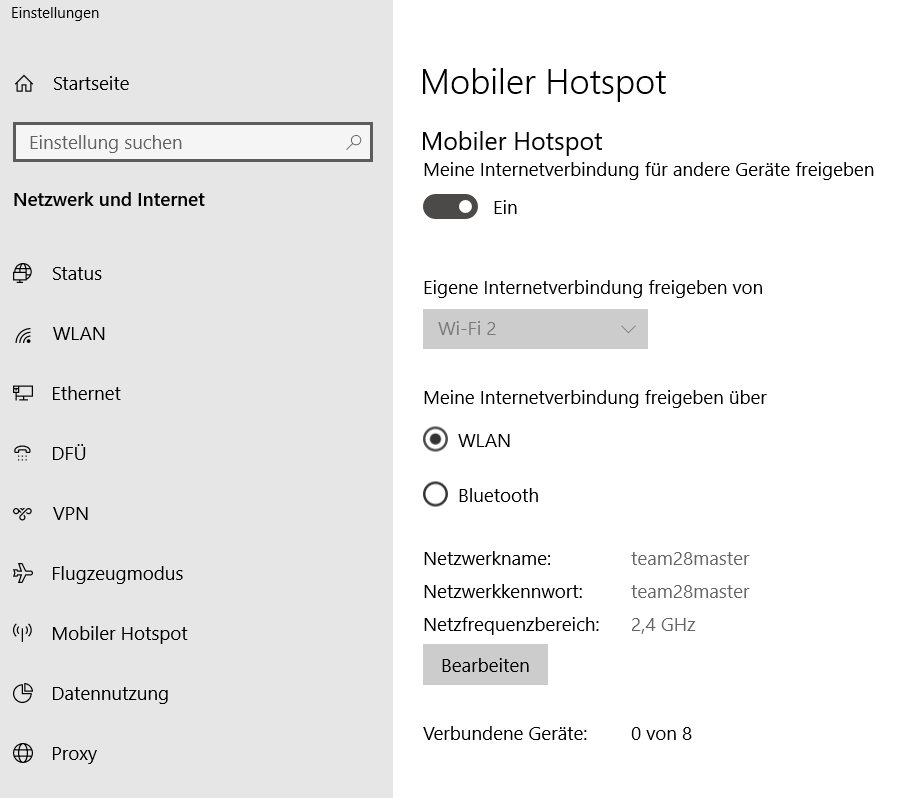
\includegraphics[width=0.75\textwidth]{HotSpot}
    \caption{WLAN Hotspot}
    \label{fig:HotSpot}
\end{figure}

Nach einigen Sekunden sollte ein Eintrag mit Informationen über den Raspi erscheinen.
Die IPv4 Adresse (Format ähnlich wie '192.168.1.12') in den Zwischenspeicher kopieren (Ctrl + C). Die IP-Adresse werden wir später noch verwenden, speichert diese in einem Textdokument (Z.B. Word). \\

Mithilfe der erhaltenen IPv4 Adresse eine Verbindung mit Putty und SHH erstellen:

\begin{itemize}
    \item Starte PuTTY
    \item Host Name (or IP address) = <IPv4> (Ctrl + V)
    \item Port = '22'
    \item Connection type = 'SSH'
    \item 'Open' klicken
\end{itemize}

Wenn wir alles richtig gemacht haben sollte nun folgendes Fenster erscheinen:
\begin{figure}[H] \centering
    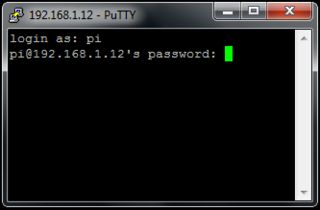
\includegraphics[width=0.5\textwidth]{PuttyRaspiLogin}
    \caption{Raspi Login Maske}
    \label{fig:Login}
\end{figure}

\begin{itemize}
    \item login = 'pi'
    \item password = 'team28'
\end{itemize}

\textbf{Raspberry Pi}\\
Von unserem Home Verzeichnis navigieren wir weiter zum Code: \\
\begin{lstlisting}
    cd team28/src/raspi
\end{lstlisting}
Von hier aus haben wir verschiedene Möglichkeiten die Applikation zu starten. \\

\textbf{Applikation}\\
Die Applikation besteht aus mehreren Modulen, welche miteinander kommunizieren. Jede dieser Module kann eigenständig ein- und ausgeschaltet werden. Zum Beispiel können wir das 'Akustik' Modul folgendermassen starten: \\
\begin{lstlisting}
    python3 /acoustic/sound.py
\end{lstlisting}
Gestoppt wird das Modul mit (Ctrl + C).\\
Für ein funktionierendes Zusammenspiel der jeweiligen Module, benötigen wir jedoch alle Module gleichzeitig. Hierführ haben wir das Bash Skript 'run-master.sh'. \\
\begin{lstlisting}
    ./run-master.sh
\end{lstlisting}
Das Skript startet zudem einen WebServer, über welchen wir die Applikation bedienen können. \\

\textbf{Web Server}\\
Der WebServer wird auf dem Port :2828 gestartet und kann jederzeit über die IP-Adresse des Raspi aufgerufen werden.
\begin{itemize}
    \item Browser starten (Firofox, Chrome, IE ...)
    \item In URL-Leiste folgendes eingeben: <IPv4>:2828/
\end{itemize}

Wenn wir alles richtig gemacht haben sollte nun folgendes Fenster erscheinen:
\begin{figure}[H] \centering
    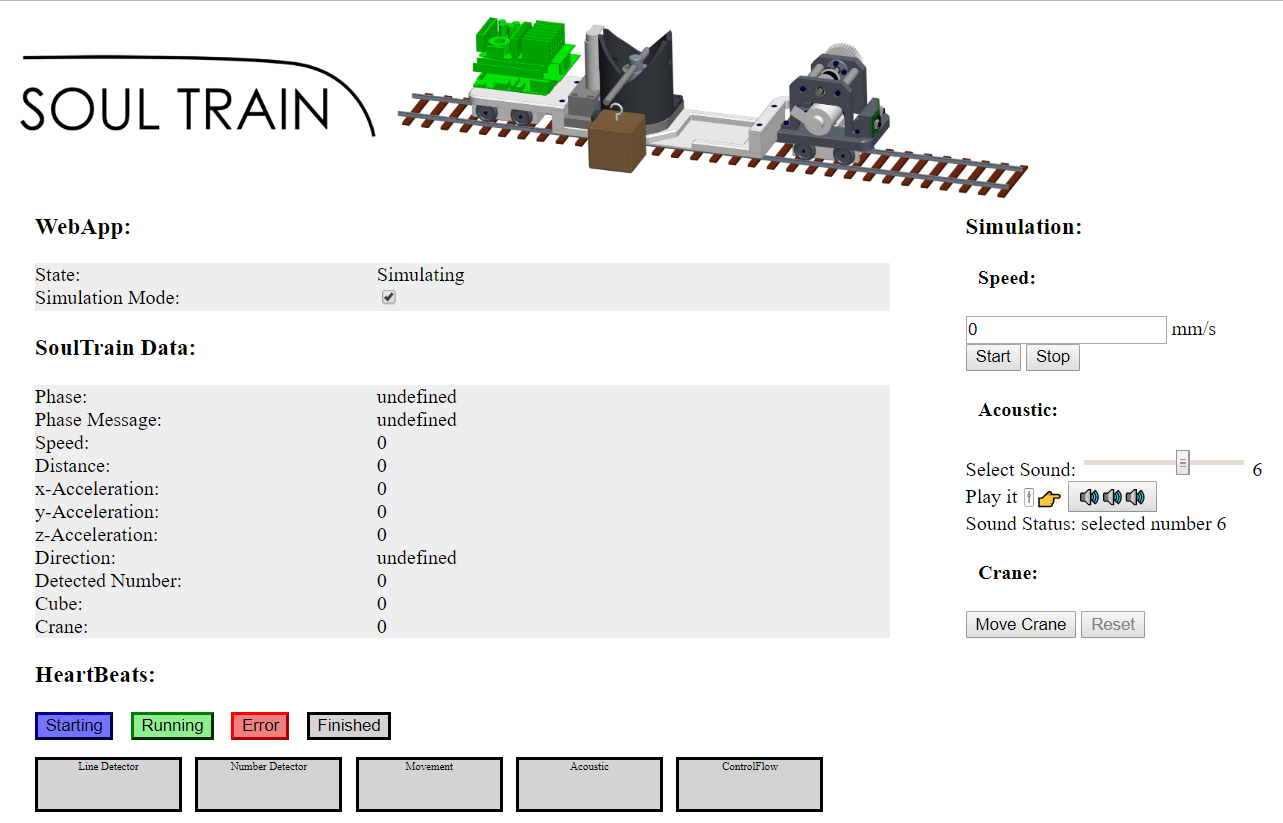
\includegraphics[width=1\textwidth]{HomeWebApp}
    \caption{Web Client}
    \label{fig:Home}
\end{figure}

\subsubsection{Web Client}
Der Web Client ist in 3 Teilbereiche aufgeteilt.
\begin{itemize}
    \item Übersicht
    \item Simulation
    \item Start
\end{itemize}
Zwischen den beiden Bereichen 'Simulation' und 'Start' kann über die Checkbox 'Simulation Mode' in der 'Übersicht' gewechselt werden.
\textbf{Übersicht}\\
\begin{figure}[H] \centering
    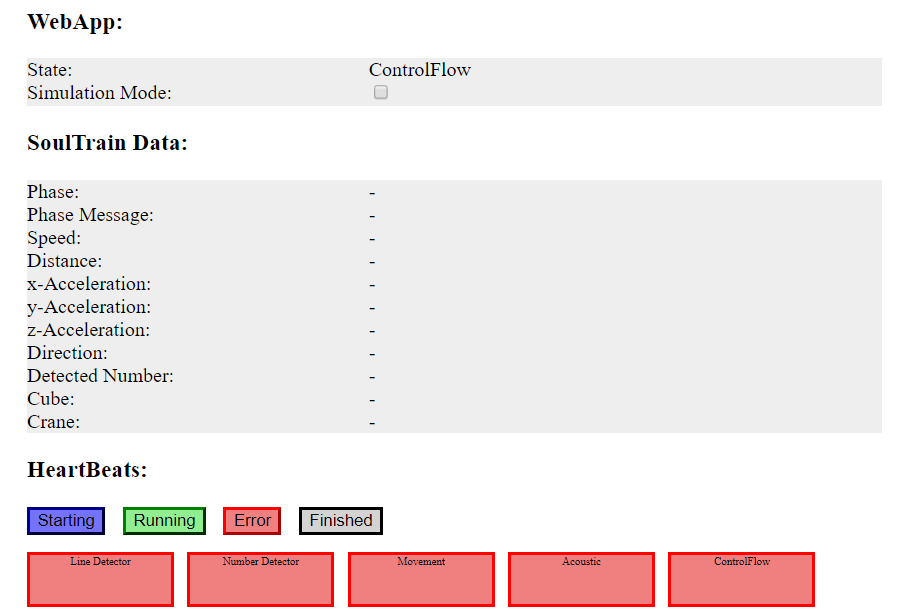
\includegraphics[width=0.75\textwidth]{UebersichtWebApp}
    \caption{Übersicht}
    \label{fig:Uebersicht}
\end{figure}
In der Übersicht werden die wichtigsten Daten in Echtzeit abgebildet. Die Daten repräsentieren Zug, Status des Zuges und dessen Umgebung. 
Man unterscheidet zwischen den Soultrain Daten und dem Hearbeat.
Soultrain Daten:

\begin{table}[H]
    \begin{tabular}{ll}
    \hline
    Phase & Die momentane Etappe des Zuges \\ \hline
    Phase Message & Nachricht welche die Phase repräsentiert\\ \hline
    Speed & Geschwindigkeit, mit welcher der Zug unterwegs ist\\ \hline
    Distance & Distanz, welche der Zug zurückgelegt hat\\ \hline
    x-Acceleration & Beschleunigung auf der x-Achse  \\ \hline
    x-Acceleration & Beschleunigung auf der y-Achse \\ \hline
    x-Acceleration & Beschleunigung auf der z-Achse \\ \hline
    Direction & Voraussichtliche Richtung der Gleise \\ \hline
    Direction Number & Nummer, welche die Richtung repräsentiert \\ \hline
    Cube & Würfel Status \\ \hline
    Crane & Kran Status \\ \hline
    \end{tabular}
\end{table}

Hearbeat:\\
Jedes Modul besitzt einen Hearbeat, welches in regelmässigen Abständen gesendet wird. Ein Modul kann folgende Zustände annehmen:
\begin{table}[H]
    \begin{tabular}{ll}
    \hline
    Starting & Während der Initialisierungsphase des Moduls \\ \hline
    Running & Solange das Modul läuft\\ \hline
    Error & Sobald ein Fehler gemeldet wird oder das Modul keinen Hearbeat mehr sendet\\ \hline
    Finished & Nach Abschluss seiner Tätigkeit\\ \hline
    \end{tabular}
\end{table} 
Folgende Module werden überwacht:
\begin{table}[H]
    \begin{tabular}{ll}
    \hline
    Line Detector & Liest die Richtung der aufkommenden Gleise während der Fahrt \\ \hline
    Number Detector & Liest die Nummern während der Fahrt\\ \hline
    Movement & Liest Geschwindigkeit und regelt die momentane Geschwindigkeit anhand dessen\\ \hline
    Acoustic & Gibt die eingelesene Nummer akustisch wieder\\ \hline
    Control Flow & Regelt den Ablauf der verschiedenen Phasen \\ \hline
    \end{tabular}
\end{table}

\textbf{Simulation}\\
\begin{figure}[H] \centering
    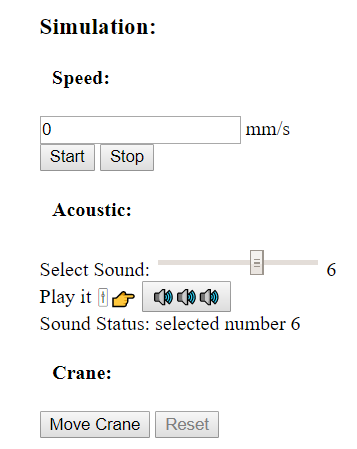
\includegraphics[width=0.5\textwidth]{SimulationWebApp}
    \caption{WebApp}
    \label{fig:Simulation}
\end{figure}
Über die Simulation kann man Komponenten während der Laufzeit testen. Folgende Komponenten kann man testen
\begin{table}[H]
    \begin{tabular}{ll}
    \hline
    Speed & Geschwindigkeit mit welcher der Zug fahren soll \\ \hline
    Acoustic & Zahl, welche die Akustische Komponente wiedergiebt\\ \hline
    Crane & Die Kranbewegung starten\\ \hline
    \end{tabular}
\end{table}
\textbf{Start}\\
\begin{figure}[H] \centering
    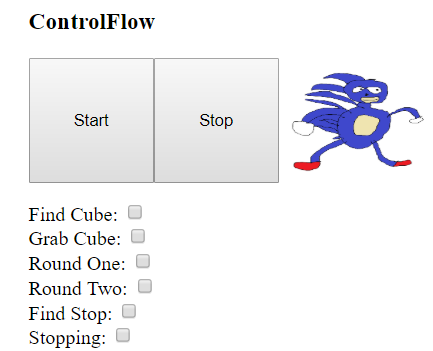
\includegraphics[width=0.5\textwidth]{StartWebApp}
    \caption{Start}
    \label{fig:Start}
\end{figure}
Start und Stop des Soultrain Ablaufs. Ausgeführt, werden nur Phasen welche gecheckt sind.
\end{document}